%%%%%%%%%%%%%%%%
%%% gen 33 %%%
%%%%%%%%%%%%%%%%

\Chapter{33}

\Verse{1}
{
	\hE{וַיִּשָּׂא יַעֲקֹב עֵינָיו וַיַּרְא וְהִנֵּה עֵשָׂו בָּא וְעִמּוֹ אַרְבַּע מֵאוֹת אִישׁ וַיַּחַץ אֶת הַיְלָדִים עַל לֵאָה וְעַל רָחֵל וְעַל שְׁתֵּי הַשְּׁפָחוֹת׃}
}
{
	\eE{
		And Jacob raised his eyes and looked, and here was Esau
		coming, and four hundred men with him. And he divided the
		children among Leah and Rachel and the two maids;
	}
}
{
	Now here's a curious section.

	So Jacob looks up and sees Esau coming with 400 guys.%
	\fC{
		Unlike Abraham and Sarah, whose new names permanently replace
		their old ones, Jacob continues to be called Jacob even after
		he is renamed Israel. This is curious.
	}

	He divides up the 12 kids between the 4 wives.
}

\Verse{2}
{
	\hE{וַיָּשֶׂם אֶת הַשְּׁפָחוֹת וְאֶת יַלְדֵיהֶן רִאשֹׁנָה וְאֶת לֵאָה וִילָדֶיהָ אַחֲרֹנִים וְאֶת רָחֵל וְאֶת יוֹסֵף אַחֲרֹנִים׃}
}
{
	\eE{
		and he placed the maids and their children first, and Leah
		and her children following, and Rachel and Joseph
		following,
	}
}
{
	He puts the maids and their kids first.
	
	Then Leah and her kids behind them.

	Then Rachel is in the back with her son Joseph,
}

\Verse{3}
{
	\hE{וְהוּא עָבַר לִפְנֵיהֶם וַיִּשְׁתַּחוּ אַרְצָה שֶׁבַע פְּעָמִים עַד גִּשְׁתּוֹ עַד אָחִיו׃}
}
{
	\eE{
		and he passed in front of them. And he bowed to the ground
		seven times until he came up to his brother.
	}
}
{
	and he passes ``before their faces'' (Heb. \heb{לפניהם}).

	And he bows to the ground seven times until Esau arrives.
}

\Verse{4}
{
	\hE{וַיָּרץ עֵשָׂו לִקְרָאתוֹ וַיְחַבְּקֵהוּ וַיִּפֹּל עַל צַוָּארָו וַיִּשָּׁקֵהוּ וַיִּבְכּוּ׃}
}
{
	\eE{
		And Esau ran to him and embraced him and fell on his neck
		and kissed him. And they wept.
	}
}
{
	Esau runs up and hugs him real hard.

	The bros kiss and cry.

%	\footnote{
%		fell on his neck. Jacob deceived his father and displaced Esau by
%		putting skins “on the smooth part of his neck” (27:16). Then there was a
%		hint that Esau would be compensated for his loss one day by the use of
%		the metaphor that “you’ll break his yoke from your neck” (27:40). And
%		now, the reconciliation between the twins is conveyed as Esau runs and
%		embraces Jacob and “fell on his neck.”
%	}
}

\Verse{5}
{
	\hE{וַיִּשָּׂא אֶת עֵינָיו וַיַּרְא אֶת הַנָּשִׁים וְאֶת הַיְלָדִים וַיֹּאמֶר מִי אֵלֶּה לָּךְ וַיֹּאמַר הַיְלָדִים אֲשֶׁר חָנַן אֱלֹהִים אֶת עַבְדֶּךָ׃}
}
{
	\eE{
		And he raised his eyes and saw the women and the children,
		and he said, “Who are these whom you have?” And he said,
		“The children with whom {\God} has graced your servant.”
	}
}
{
	He looks up and sees all the women and kids.

	And he's like ``Who've you got here?''

	He says it's his kids.
}

\Verse{6}
{
	\hE{וַתִּגַּשְׁןָ הַשְּׁפָחוֹת הֵנָּה וְיַלְדֵיהֶן וַתִּשְׁתַּחֲוֶיןָ׃}
}
{
	\eE{
		And the maids came over, they and their children, and
		bowed.
	}
}
{
	Bilhah and Zilpah and the kids bow.
}

\Verse{7}
{
	\hE{וַתִּגַּשׁ גַּם לֵאָה וִילָדֶיהָ וַיִּשְׁתַּחֲווּ וְאַחַר נִגַּשׁ יוֹסֵף וְרָחֵל וַיִּשְׁתַּחֲווּ׃}
}
{
	\eE{
		And Leah and her children, too, came over, and they bowed.
		And then Joseph and Rachel came over, and they bowed.
	}
}
{
	Then Leah and her kids do the thing.

	Then Rachel's son Joseph and Rachel herself do it.
%	\footnote{
%		Joseph and Rachel came over. Leah, Bilhah, and Zilpah are mentioned
%		before their children, but Joseph is mentioned before Rachel, yielding a
%		picture of him approaching ahead of her. In his favor, we might take
%		this as a protective gesture toward his mother. Alternatively, we might
%		take this as consistent with the next picture we shall have of his early
%		years: seeing himself in a special status relative to his family.
%	}
}

\Verse{8}
{
	\hE{וַיֹּאמֶר מִי לְךָ כּל הַמַּחֲנֶה הַזֶּה אֲשֶׁר פָּגָשְׁתִּי וַיֹּאמֶר לִמְצֹא חֵן בְּעֵינֵי אֲדֹנִי׃}
}
{
	\eE{
		And he said, “Who is all this camp of yours that I met?”
		And he said, “To find favor in my lord’s eyes.”
	}
}
{
	\aB{
	And he's like ``Who was all that?''

	And he's like ``To find favor in my lord's eyes.''

	Not clear what happened here.
	}

	\aA{
	Presumably Esau here is saying something like:

	``What's the deal with all those gift from before?''

	If so, Jacob's response makes sense.
	}
}

\Verse{9}
{
	\hE{וַיֹּאמֶר עֵשָׂו יֶשׁ לִי רָב אָחִי יְהִי לְךָ אֲשֶׁר לָךְ׃}
}
{
	\eE{
		And Esau said, “I have a great deal, my brother. Let
		what’s yours be yours.”
	}
}
{
	So Esau's like
	``Bro I've got enough stuff, you don't need to give me presents.''

%	\footnote{
%		Let what’s yours be yours. Esau graciously refuses Jacob’s gift. Then
%		Jacob presses him to accept it. Then Esau takes it. As in the episode of
%		Abraham’s purchase of the tomb for Sarah, and Lot’s offering his
%		daughters to the people of Sodom, Jacob and Esau are going through the
%		classic Near Eastern conventions, which continue to this day.
%	}
}

\Verse{10}
{
	\hE{וַיֹּאמֶר יַעֲקֹב אַל נָא אִם נָא מָצָאתִי חֵן בְּעֵינֶיךָ וְלָקַחְתָּ מִנְחָתִי מִיָּדִי כִּי עַל כֵּן רָאִיתִי פָנֶיךָ כִּרְאֹת פְּנֵי אֱלֹהִים וַתִּרְצֵנִי׃}
}
{
	\eE{
		And Jacob said, “Don’t. If I’ve found favor in your eyes,
		then you’ll take my offering from my hand, because on
		account of this I’ve seen your face—like seeing {\God}’s
		face!—and you’ve accepted me.
	}
}
{
	Jacob's like ``Please I insist.''

	Then he says this curious thing about how Esau's face is like The Face of God.

	Which is why he named the place ``Peni El'' in the previous chapter
	after the wrestling scene.

%	\footnote{
%		I’ve seen your face—like seeing God’s face. Esau has no idea just how
%		literally this is meant. Jacob had prayed for help because he was afraid
%		of Esau. Then he had the encounter after which he said, “I’ve seen God
%		face-to-face.” And this, presumably, enabled him to face his brother.
%		Esau may take Jacob’s words as a great compliment, but they actually
%		convey that, after facing God, one is certainly able to face any human.
%	}
}

\Verse{11}
{
	\hE{קַח נָא אֶת בִּרְכָתִי אֲשֶׁר הֻבָאת לָךְ כִּי חַנַּנִי אֱלֹהִים וְכִי יֶשׁ לִי כֹל וַיִּפְצַר בּוֹ וַיִּקָּח׃}
}
{
	\eE{
		Take my blessing that’s been brought to you, because {\God}
		has been gracious to me and because I have everything.”
		And he pressed him, and he took it.
	}
}
{
	Hey remember in the previous scene where \textsl{someone} said:
	
	``I won't let you go until you give me your blessing.''

	Ok so here Jacob's like ``Take my blessing.''

	Also recall that before this scene, the bros last scene together was
	the ``Jacob steals the blessing'' scene.%
	\fB{Also known as The Blinding of Isaac among the erudite.}

	Jacob insists, so Esau accepts.
%	\footnote{
%		Take my blessing. It was Jacob’s taking of Esau’s blessing that led to
%		the brothers’ separation. His description now of what he is offering as
%		“my blessing” suggests that it is an act of compensation for what he did
%		to Esau twenty years earlier. Unlike biblical interpreters who try to
%		defend Jacob’s earlier actions, Jacob himself is pictured as (1) not
%		trying to make any excuses, and (2) trying to make amends.
%	}
}

\Verse{12}
{
	\hE{וַיֹּאמֶר נִסְעָה וְנֵלֵכָה וְאֵלְכָה לְנֶגְדֶּךָ׃}
}
{
	\eE{
		And he said, “Let’s travel, and let’s go. And let me go
		alongside you.”
	}
}
{
	So he (presumably Esau) is all happy that they've finally made amends,
	and he suggests they hang out and go on adventures together.
}

\Verse{13}
{
	\hE{וַיֹּאמֶר אֵלָיו אֲדֹנִי יֹדֵעַ כִּי הַיְלָדִים רַכִּים וְהַצֹּאן וְהַבָּקָר עָלוֹת עָלָי וּדְפָקוּם יוֹם אֶחָד וָמֵתוּ כּל הַצֹּאן׃}
}
{
	\eE{
		And he said to him, “My lord knows that the children are
		weak and the nursing sheep and oxen are with me, and
		they’ll drive them one day and all the sheep will die.
	}
}
{
	So he (presumably Jacob) is like ``Oh gosh, well you know I'd love to,
	best bro, heh, but the kids are real young, and if we let you come
	along then like, I dunno, um, all the sheep\footnote{
	Lit. \heb{רחל}s and \heb{איל}s.
	} might die.''
}

\Verse{14}
{
	\hE{יַעֲבר נָא אֲדֹנִי לִפְנֵי עַבְדּוֹ וַאֲנִי אֶתְנָהֲלָה לְאִטִּי לְרֶגֶל הַמְּלָאכָה אֲשֶׁר לְפָנַי וּלְרֶגֶל הַיְלָדִים עַד אֲשֶׁר אָבֹא אֶל אֲדֹנִי שֵׂעִירָה׃}
}
{
	\eE{
		Let my lord pass on in front of his servant; and I, let me
		move along at my pace required by the task that’s before
		me and required by the children until I come to my lord at
		Seir.”
	}
}
{
	You go on ahead.

	I'll go at my own speed.

	For the kids.

	I'll meet you in Harrisburg.\fC{Seir (\heb{שֵׂעִיר}) means ``hairy'' or ``shaggy,'' from \heb{שֵׂעָר}, ``hair.'' Esau himself is described as \heb{שָׂעִר}, ``hairy'' (27:11). Presumably this is what the text meant here.}
}

\Verse{15}
{
	\hE{וַיֹּאמֶר עֵשָׂו אַצִּיגָה נָּא עִמְּךָ מִן הָעָם אֲשֶׁר אִתִּי וַיֹּאמֶר לָמָּה זֶּה אֶמְצָא חֵן בְּעֵינֵי אֲדֹנִי׃}
}
{
	\eE{
		And Esau said, “Let me set with you some of the people who
		are with me.” And he said, “Why have I found favor in my
		lord’s eyes?”
	}
}
{
	Esau's like ``Here take some of my guys.''

	Jacob is confused about why Esau's being so nice to him.
%	\footnote{
%		Why have I found favor in my lord’s eyes? Jacob seems to be saying, “No,
%		no, I don’t deserve this kindness from you,” which appears to be an
%		extremely polite way of declining Esau’s offer. Understandably, this
%		offer to post some men with Jacob is not attractive to him: Jacob has
%		just told Esau that he will meet him in Seir, but in fact the next two
%		verses report that Esau goes back to Seir but Jacob goes to Sukkot!
%	}
}

\Verse{16}
{
	\hE{וַיָּשׁב בַּיּוֹם הַהוּא עֵשָׂו לְדַרְכּוֹ שֵׂעִירָה׃}
}
{
	\eE{And Esau went back on his way to Seir that day,}
}
{
	So Esau goes to Seir, where Jacob just promised to meet him.

	Meanwhile, while Esau is patiently waiting...
}

\Verse{17}
{
	\hE{וְיַעֲקֹב נָסַע סֻכֹּתָה וַיִּבֶן לוֹ בָּיִת וּלְמִקְנֵהוּ עָשָׂה סֻכֹּת עַל כֵּן קָרָא שֵׁם הַמָּקוֹם סֻכּוֹת׃}
}
{
	\eE{
		and Jacob traveled to Sukkot. And he built a house for
		himself and made booths for his cattle. On account of this
		he called the place’s name Sukkot.
	}
}
{
	Jacob's like ``Fukkot'' and heads off to Sukkot.

	\begin{center}
		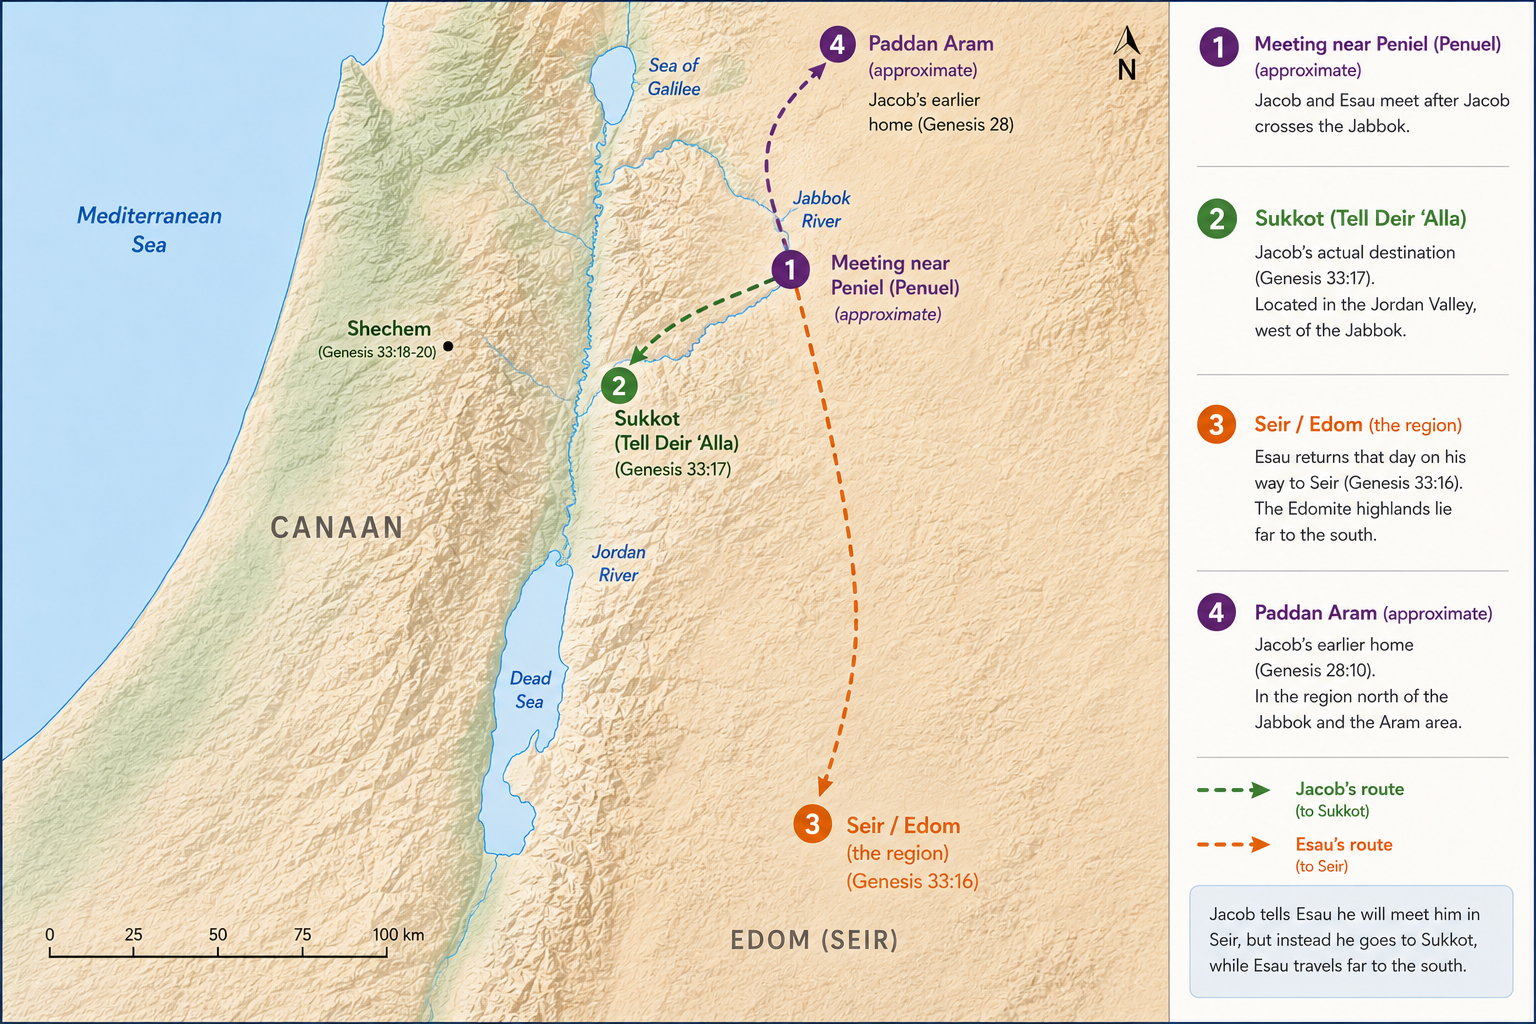
\includegraphics[width=0.9\linewidth]{img/genesis-33-map.png}
	\end{center}

	Then he builds a house for himself and some Sukkahs for his cows.

	Which is the reason why we Sukkot to this day.\fB{
		A well known holiday where you build a Sukkah and you
		hold a lemon and shake a branch or something, and we
		also get the day off work. That's why I can't come in
		to work today boss man. Cuz Sukkot. No no that's not
		what I said don't get mad. I said Sukkot. And there's
		not just one big Sukkah, everyone makes their own
		Sukkah, so there's a lot of them going up around this
		time of year boss man, you could almost say there's a
		Sukkah born every minute. Anyways gotta run. I'll see
		ya in a week.
	}
}

\Verse{18}
{
	\hE{וַיָּבֹא יַעֲקֹב שָׁלֵם עִיר שְׁכֶם}
	\hR{אֲשֶׁר בְּאֶרֶץ כְּנַעַן בְּבֹאוֹ מִפַּדַּן אֲרָם}
	\hE{וַיִּחַן אֶת פְּנֵי הָעִיר׃}
}
{
	\eE{
		And Jacob came, safe, to the city of Shechem,
	}
	\eR{
		which was in the land of Canaan, when he was coming from Paddan Aram,
	}
	\eE{
		and camped in front of the city.
	}
}
{
	Jacob comes, unharmed, to Shechem \eR{when he was coming from Paddan Aram}
	and he camps in front of the city.
}

\Verse{19}
{
	\hE{וַיִּקֶן אֶת חֶלְקַת הַשָּׂדֶה אֲשֶׁר נָטָה שָׁם אהֳלוֹ מִיַּד בְּנֵי חֲמוֹר אֲבִי שְׁכֶם בְּמֵאָה קְשִׂיטָה׃}
}
{
	\eE{
		And he bought the section of field in which he pitched his
		tent from the hand of the sons of Hamor, father of
		Shechem, for a hundred qesita.
	}
}
{
	And he buys some land in Shechem from a guy named Shechem,
	and his brothers, who are the sons of a guy named Ass, and he
	buys it fair and square, for a hundred qesita.

	We don't know how much a qesita is.
	
	The Septuagint\fC{
		The Septuagint (LXX) is an ancient translation of the Hebrew Bible
		into Greek, begun several centuries before our oldest surviving
		complete Hebrew manuscripts, so its wording can sometimes preserve
		evidence for an older Hebrew text or interpretation.
	} thinks it's sheep.

	Just make a note of that for now, we'll learn more in the coming chapter.
}

\Verse{20}
{
	\hE{וַיַּצֶּב שָׁם מִזְבֵּחַ וַיִּקְרָא לוֹ אֵל אֱלֹהֵי יִשְׂרָאֵל׃}
}
{
	\eE{
		And he set up an altar there and called it “El, {\God} of
		Israel.”
	}
}
{
	So Jacob aka Israel sets up an altar, and calls it

	El, oh El.\footnote{
		Lit. \heb{ל ו אל} in the original.
	}

	Israel.

	Right, on to Shechem.
}
